
%(BEGIN_QUESTION)
% Copyright 2010, Tony R. Kuphaldt, released under the Creative Commons Attribution License (v 1.0)
% This means you may do almost anything with this work of mine, so long as you give me proper credit

Sketch connecting wires such that the relay will select one of two different thermocouples to send millivoltage signals to a temperature indicator.  Use the following schematic diagram as a guide:

$$\includegraphics[width=15.5cm]{i04588x01.eps}$$

\underbar{file i04588}
%(END_QUESTION)





%(BEGIN_ANSWER)

$$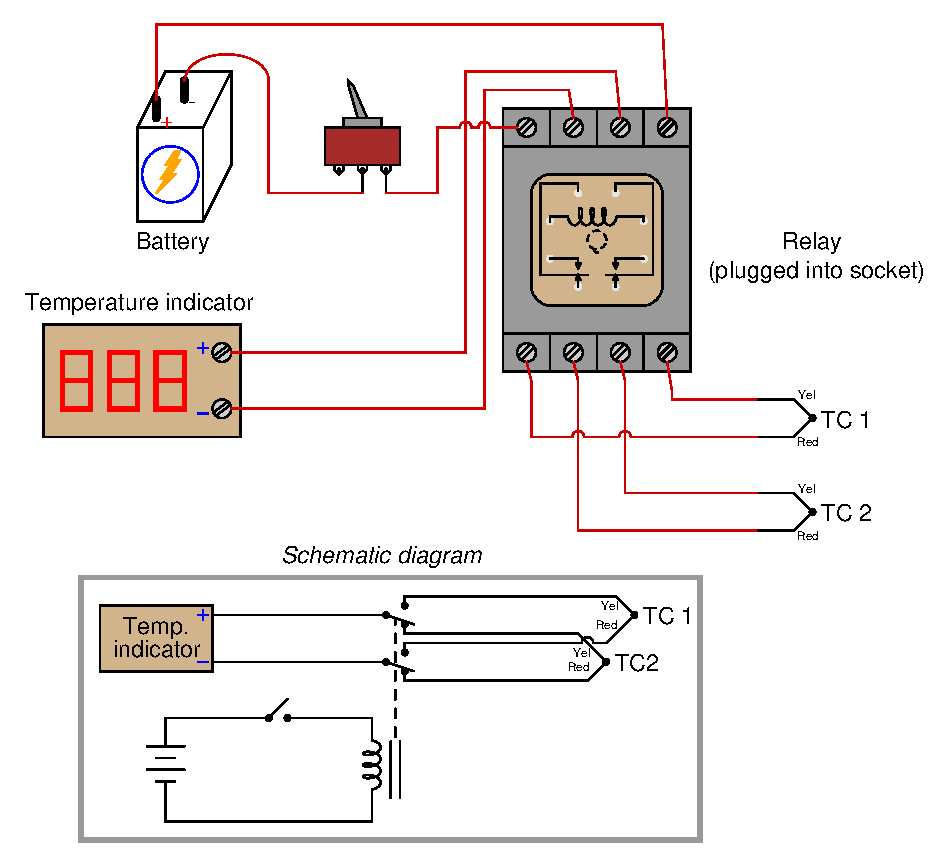
\includegraphics[width=15.5cm]{i04588x02.eps}$$

%(END_ANSWER)





%(BEGIN_NOTES)

Note how a schematic diagram was provided for you, to help you determine where each and every wire should go.  In real-life situations, you may not be given any schematic diagram at all.  In such cases, it is an excellent problem-solving strategy to first sketch your own schematic diagram, before attempting to sketch a pictorial diagram or connect real wires to the devices.  The concept here is that schematic diagrams are much easier to interpret and understand than pictorial diagrams where wires tend to cross over each other more, and where components are not always optimally placed.

%INDEX% Pictorial circuit review (relay circuit)

%(END_NOTES)


